\documentclass[border=6pt]{standalone}
\usepackage{tikz}
\usetikzlibrary{positioning,arrows.meta,fit,backgrounds,shapes.geometric}
\definecolor{navy}{HTML}{161E29}
\definecolor{slate}{HTML}{2E3D50}
\definecolor{slatefill}{HTML}{E9EDF2}
\definecolor{accent}{HTML}{B45309}
\definecolor{accentfill}{HTML}{FEF3C7}
\definecolor{edge}{HTML}{51647D}
\begin{document}
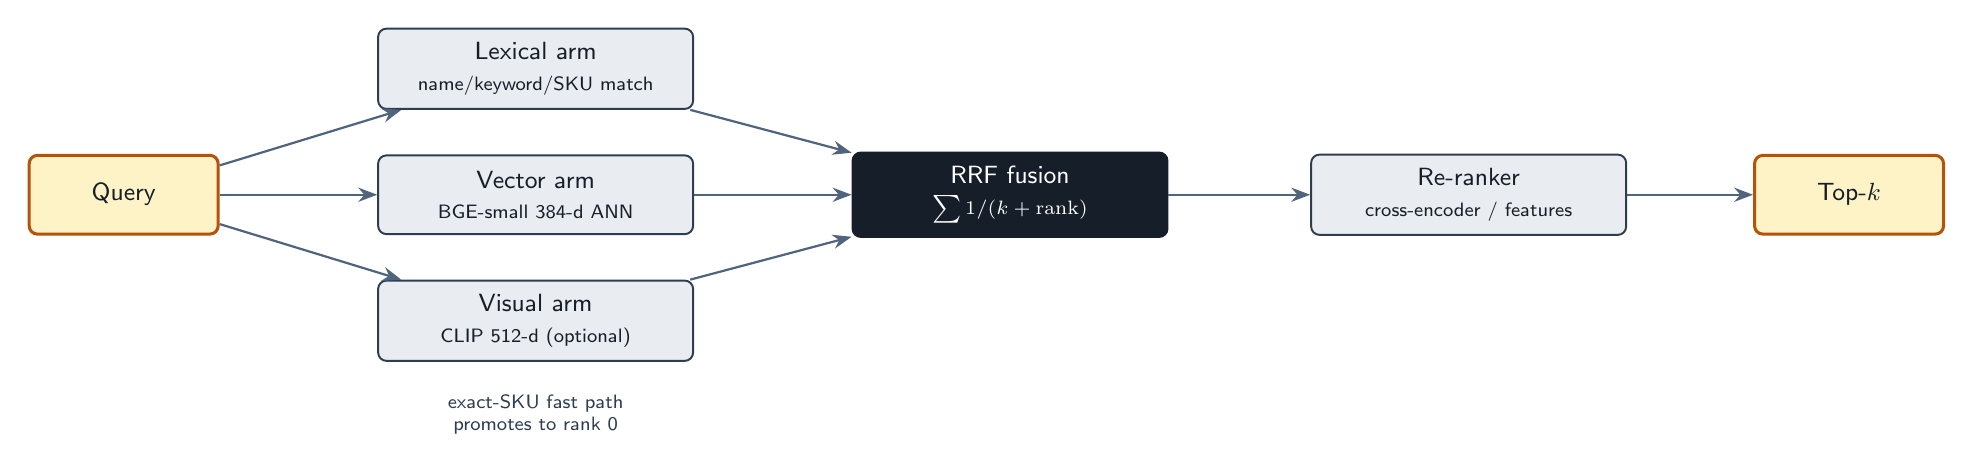
\begin{tikzpicture}[
  font=\sffamily\small,
  box/.style={rounded corners=3pt, draw=slate, line width=0.7pt, fill=slatefill, text=navy, align=center, inner sep=5pt, minimum height=10mm, minimum width=40mm},
  dark/.style={box, fill=navy, draw=navy, text=white},
  acc/.style={box, draw=accent, line width=1.1pt, fill=accentfill, text=navy, minimum width=24mm},
  lbl/.style={font=\sffamily\scriptsize, text=slate},
  arr/.style={-{Stealth[length=2.4mm]}, line width=0.8pt, draw=edge},
]
\node[acc] (q) {Query};
\node[box, right=20mm of q, yshift=16mm] (lex) {Lexical arm\\{\scriptsize name/keyword/SKU match}};
\node[box, right=20mm of q] (vec) {Vector arm\\{\scriptsize BGE-small 384-d ANN}};
\node[box, right=20mm of q, yshift=-16mm] (vis) {Visual arm\\{\scriptsize CLIP 512-d (optional)}};
\node[dark, right=20mm of vec] (rrf) {RRF fusion\\{\scriptsize $\sum 1/(k+\mathrm{rank})$}};
\node[box, right=18mm of rrf] (rr) {Re-ranker\\{\scriptsize cross-encoder / features}};
\node[acc, right=16mm of rr] (out) {Top-$k$};
\draw[arr] (q) -- (lex);
\draw[arr] (q) -- (vec);
\draw[arr] (q) -- (vis);
\draw[arr] (lex) -- (rrf);
\draw[arr] (vec) -- (rrf);
\draw[arr] (vis) -- (rrf);
\draw[arr] (rrf) -- (rr);
\draw[arr] (rr) -- (out);
\node[lbl, below=3mm of vis, text width=44mm, align=center] {exact-SKU fast path promotes to rank 0};
\end{tikzpicture}
\end{document}
